\documentclass[14pt]{extreport}
\usepackage{authblk}
\usepackage[utf8]{vietnam}
\usepackage{amsmath}
\usepackage{amsfonts}
\usepackage{amssymb}
\usepackage{graphicx}
\usepackage{longtable}
\usepackage{multirow}
\usepackage[english]{babel}
\usepackage[utf8]{inputenc}
\usepackage{fancyhdr}
\usepackage{float}
\usepackage[table,xcdraw]{xcolor}

%---------------------------------------------------------
\pagestyle{fancy}
\fancyhf{}
\rhead{\rightmark}
\lhead{\leftmark}
\rfoot{Page \thepage}
\title{Đồ án socket}
\author{Vu Cong Duy - 19120212\\ Nguyen Hoang Anh Kiet - 19120266}

\date{December 2020}


\begin{document}
\maketitle
\chapter{Socket}
\section{Lựa chọn giao thức tầng ứng dụng}

Trước khi bắt đầu lập trình một chương trình ứng dụng socket mạng, việc quan trọng nhất chính là việc chọn giao thức tầng transport mà ứng dụng đó sẽ dùng.\cite{1} Bởi đây là nơi sâu nhất mà một lập trình viên có thể can thiệp, giao thức tầng transport sẽ ảnh hưởng tới toàn bộ chương trình.

Có 2 giao thức phổ biến : UDP và TCP. Ta có thể thấy, việc truyền tải dữ liệu một trang web đòi hỏi phải có độ tin cậy cao. Vì vậy, giao thức truyền dữ liệu TCP sẽ là phù hợp hơn cho chương trình socket này. Thật vậy, giao thức HTTP (giao thức về truyền dữ liệu web) ở tầng application cũng đã chọn giao thức TCP để truyền tải dữ liệu trang web.


\section{Mô hình triển khai}

Về cơ bản, mọi chương trình sử dụng giao thức TCP  đều có mô hình Client-Server triển khai như sau.
\begin{center}
    \begin{figure}[H]
    \begin{center}
     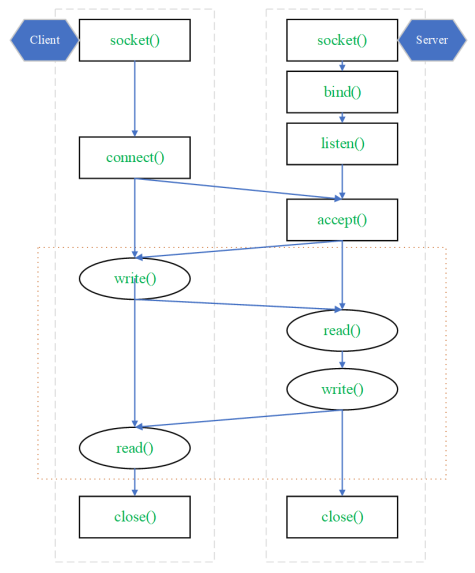
\includegraphics[scale=.65]{mo hinh trien khai tcp.PNG}
    \end{center}
    \caption{Mô hình Client-Server triển khai theo giao thức tcp}
    \label{refhinh1}
    \end{figure}
\end{center}

Trong đồ án này, chương trình Client chính là web browser đã được lập trình sẵn, vì vậy phần này sẽ được duyệt nhanh và chú trọng hơn vào phần lập trình socket Server.
\subsection{Giai đoạn 1: Khởi tạo socket cho server}



Với server:

-Server tạo socket bằng lệnh {\bf socket()}. Với ngôn ngữ python, việc này thực hiện bằng hàm socket() trong thư viện socket (đã được import từ trước).Hàm socket còn có thể truyền tham số đầu vào như giao thức địa chỉ IP (IPv4 và IPv6) và giao thức tầng transport (UDP và TCP). Nếu không truyền tham số, hàm tự động tạo một socket có giao thức IPv4/TCP. Những giá trị hằng cho các tham số trên được quy định như hình dưới.

\begin{center}
    \begin{figure}[H]
    \begin{center}
     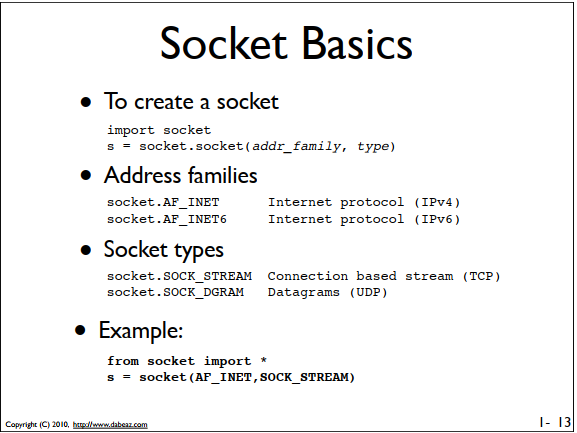
\includegraphics[scale=.8]{gia tri tham so cho ham socket.PNG}
    \end{center}
    \caption{Giá trị các tham số cho hàm socket \cite{2}}
    \label{refhinh3}
    \end{figure}
\end{center}

- Sau đó, server gán socket này một port ( ở trường hợp này là port 80) và địa chỉ IP của server (ở đây là máy đang chạy chương trình). Trong ngôn ngữ python, hành động này được thực hiện bằng hàm {\bf bind()}. Tham số truyền vào chính là một tuple biểu diễn cặp địa chỉ IP - port mà chương trình muốn gán cho socket. Địa chỉ IP được viết dưới kiểu dữ liệu chuỗi, trong khi port là kiểu dữ liệu số nguyên.

\begin{center}
    \begin{figure}[H]
    \begin{center}
     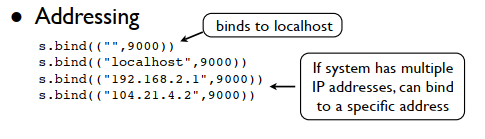
\includegraphics[scale=.8]{lenh bind.PNG}
    \end{center}
    \caption{Minh họa cho hàm bind \cite{2}}
    \end{figure}
\end{center}

- Cuối cùng, cho sever bắt đầu lắng nghe yêu cầu bằng lệnh {\bf listen()}. \cite{2}Tham số đầu có kiểu dữ liệu số nguyên, phụ thuộc vào số kết nối trong hàng chờ được phép có (hoàn toàn không phụ thuộc vào số client tối đa).

\begin{center}
    \begin{figure}[H]
    \begin{center}
     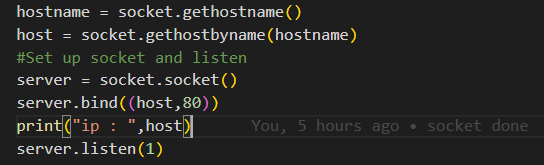
\includegraphics[scale=.8]{set up socket server.PNG}
    \end{center}
    \caption{Các bước thiết lập socket Server hoàn chỉnh để sẵn sàng lắng nghe yêu cầu từ Client}
    \end{figure}
\end{center}

\subsection{Giai đoạn 2: Khởi tạo socket cho client }
Việc khởi tạo socket cho client cũng có nhiều điểm tương đồng với tạo socket cho server.

- Client yêu cầu tạo một socket với lệnh {\bf socket()}. Tương ứng với lệnh socket() của server, lệnh tạo socket từ client cũng yêu cầu phương thức IP và phương thức của tầng transport. Web browser sẽ mặc định dùng giao thức TCP.
-Sau khi tạo socket, client sẽ kết nối socket vừa tạo đến socket của server, với lệnh {\bf connect()}. Lệnh này có tham số đầu vào tương đồng với lệnh {\bf bind()} của server khi đều yêu cầu địa chỉ IP và port của socket server. Với web browser, các nhà phát triển đã lập trình tham số địa chỉ IP chính là địa chỉ IP (của tên miền nếu user nhập tên miền) nhập trên thanh truy cập, còn port mặc định là 80. 

Ngay sau khi client thực hiện lệnh {\bf connect()} thì tại server:
-Server nhận được thông điệp yêu cầu kết nối từ lệnh connect() thì thực hiện lệnh chấp nhận bằng lệnh {\bf accept()}, đồng thời cũng tạo ra một socket mới mà việc {\bf truyền thông điệp response - request sẽ diễn ra trên socket này} (chứ không trên socket ban đầu mà server đã tạo!). Trong ngôn ngữ Python, method connect() sẽ trả giá trị là một tuple gồm socket mới và địa chỉ IP của client. 


\subsection{Giai đoạn 3: Trao đổi thông điệp giữa client và server}
Hai thao tác cơ bản trong giai đoạn này là gửi và nhận thông tin. Trong ngôn ngữ python, các hàm gửi và nhận dưới dạng method của đối tượng socket lần lượt là : 

{\bf send()/sendall()} : biến đầu vào là dữ liệu được mã hóa nhị phân

{\bf recieve()}: biến đầu vào là kích thước biến nhận dữ liệu, dữ liệu nhận được là dữ liệu nhị phân, muốn đọc hoặc xử lý thì phải mã hóa.

\begin{center}
    \begin{figure}[H]
    \begin{center}
     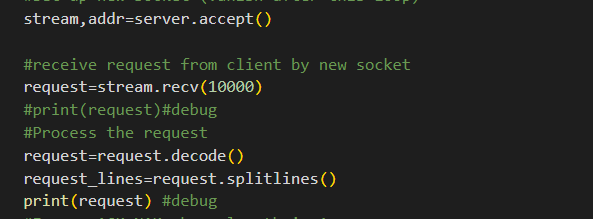
\includegraphics[scale=.8]{server accept va recieve.PNG}
    \end{center}
    \caption{Server thực hiện lệnh accecpt và recieve}
    \end{figure}
\end{center}

Chi tiết phần trao đổi thông điệp giữa client và server sẽ được trình bày chi tiết ở Chương 2.

\subsection{Giai đoạn 4: Kết thúc phiên làm việc}
Sau khi trao đổi thông điệp kết thúc, server thực hiện đóng socket mà dùng để trao đổi thông tin với client và client cũng làm điều tương tự. Lưu ý : socket server đóng là socket phát sinh bởi hàm connect(), không phải là socket tạo từ đầu. Trong thực tế server luôn ở trong trạng thái hoạt động nên socket server tạo từ đầu sẽ không bao giờ đóng.

Ở ngôn ngữ python, socket được đóng bằng lệnh {\bf close()}, không yêu cầu tham số đầu vào.

\chapter{Thông điệp HTTP}
\section{Cấu trúc request}
Một request hoàn chỉnh có rất nhiều trường dữ liệu, nhưng về cơ bản, phần quan trọng nhất để một request có thể xử lý được là :

{\it <tên method> <đường dẫn file> <tên phiên bản http>}

{\it Host : <địa chỉ IP của client>}

.
.
.

{\it Transfer-encoding:<cách thức encode>}\\

{\it <data>}

\begin{center}
    \begin{figure}[H]
    \begin{center}
     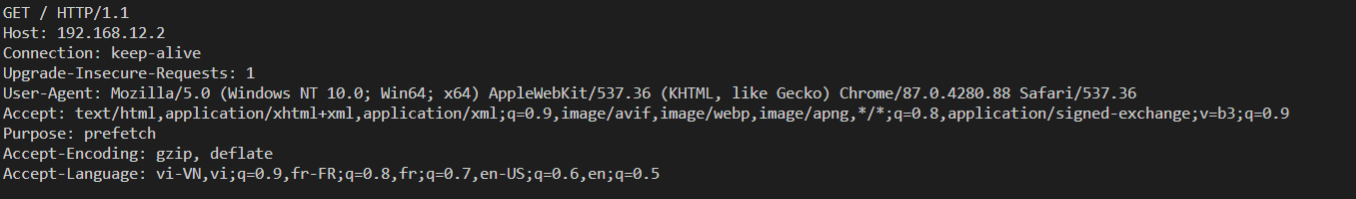
\includegraphics[scale=.8]{client request.PNG}
    \end{center}
    \caption{Một request cơ bản điển hình}
    \end{figure}
\end{center}

Những phần khác là những chi tiết mà để xử lý chúng đòi hỏi người cài đặt phải có kỹ thuật cao. Trong khuôn khổ đồ án này ta sẽ không bàn tới.
\section{Loại kết nối}
\cite{1} Khi tương tác server-client diễn ra trên giao thức TCP, người phát triển ứng dụng cần đưa ra một quyết định quan trọng: mỗi cặp request/response (yêu cầu/ phản hồi) sẽ sử dụng một kết nối TCP {\bf chung} hay mỗi cặp cặp request/response sẽ sử dụng một kết nối TCP {\bf riêng}. Theo cách ban đầu, ứng dụng được cho là sử dụng kết nối thường trực [persistent connections], còn theo cách sau thì gọi là kết nối không thường trực [non-persisitent connection].

Do kết nối thường trực có cách cài đặt tương đối khó khăn, chương trình trong đồ án này sẽ lựa chọn non-persistent connections. Vì vậy, mỗi đối tượng sẽ được gửi trong một phiên giao tiếp TCP giữa client-server, sau khi gửi xong thì kết nối TCP này cũng tự động ngắt kết nối.

Theo đó, mỗi một object trong một file html ( bao gồm cả file html) sẽ được chuyển từ server đến client trong từng phiên riêng. Sau khi kết thúc việc truyền 1 object, server sẽ đóng socket truyền object đó bằng lệnh close().
\section{CTE}
Đồ án lựa chọn một cách thức encode đơn giản nhưng hiệu quả đó chính là chunked transfer encoding (gọi tắt là CTE). Theo đó một thông điệp chứa dữ liệu mà client yêu cầu sẽ được cắt nhỏ ra từng chunk (từng khối) rồi gửi từng phần đi thay vì gửi hết tất cả dữ liệu trong một lần gửi.
\section{Cấu trúc response}

\subsection{Method của request là GET}
Dựa vào kiến thức về CTE ở trên, ta tiến hành xây dựng cấu trúc response.\\
{\it HTTP/1.1 200 OK}\\
{\it Content-Type: <tên kiểu file chuyền>}\\
{\it Transfer-encoding:Chunked-encoding}\\
{\it <kích thước chunk01 viết dưới dạng hex> \textbackslash r\textbackslash n }\\
{\it <data của chunk01>\textbackslash r\textbackslash n}\\
{\it <kích thước chunk02 viết dưới dạng hex> \textbackslash r\textbackslash n }\\
{\it <data của chunk02>\textbackslash r\textbackslash n}\\

.
.
.\\
{\it 0 \textbackslash r\textbackslash n }(chunk gửi cuối cùng luôn là chunk rỗng nên kích thước là 0)\\
{\it <data của chunk cuối >\textbackslash r\textbackslash n}(rỗng)\\
{\it \textbackslash r\textbackslash n}(dấu hiệu kết thúc việc gửi chunk, lúc này client sẽ tự đóng socket)

\begin{center}
    \begin{figure}[H]
    \begin{center}
     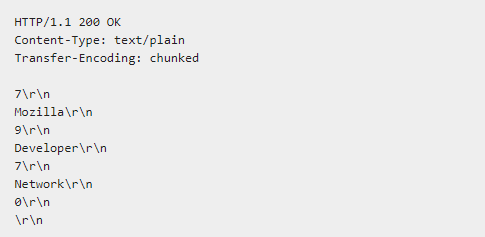
\includegraphics[scale=.8]{CTE example.PNG}
    \end{center}
    \caption{Ví dụ cho response chuyền dữ liệu theo phương thức CTE\cite{3}}
    \end{figure}
\end{center}

Chi tiết cách cài đặt : Lần send đầu tiên, server sẽ tiến hành send header. Sau đó, server sẽ thực hiện lặp: lần lượt đọc dữ liệu file cần gửi, send kích thước chunk, rồi send data của chunk cho đến khi dữ liệu của file được đọc hết. Sau đó send chuỗi \textbackslash r\textbackslash n để client biết kết thúc chunk và đóng socket.

Lưu ý: để xử lý trường hợp client yêu cầu file không có thực, ta sẽ kiểm tra liệu file có tồn tại không bằng cách mở và đóng file. Nếu xảy ra lỗi, ta sẽ gửi lại 404 Not found response (sẽ được trình bày ở phần sau).
\begin{center}
    \begin{figure}[H]
    \begin{center}
     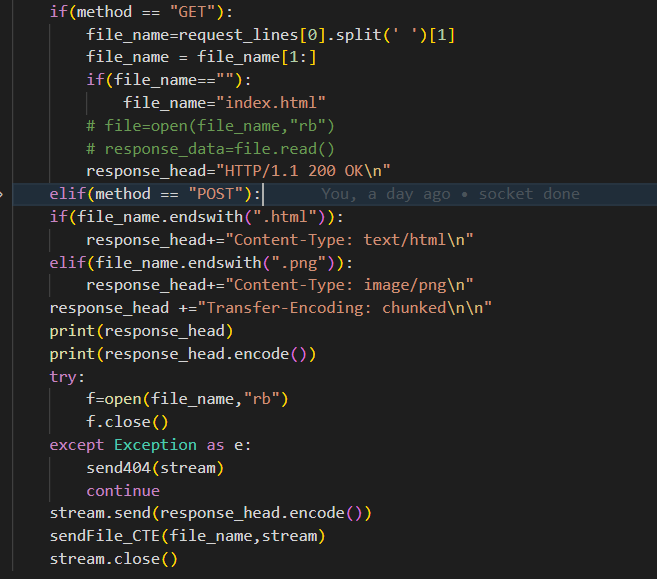
\includegraphics[scale=1.0]{GET implement.PNG}
    \end{center}
    \caption{Gửi phần header cho client trước khi gửi phần data}
    \end{figure}
\end{center}

\begin{center}
    \begin{figure}[H]
    \begin{center}
     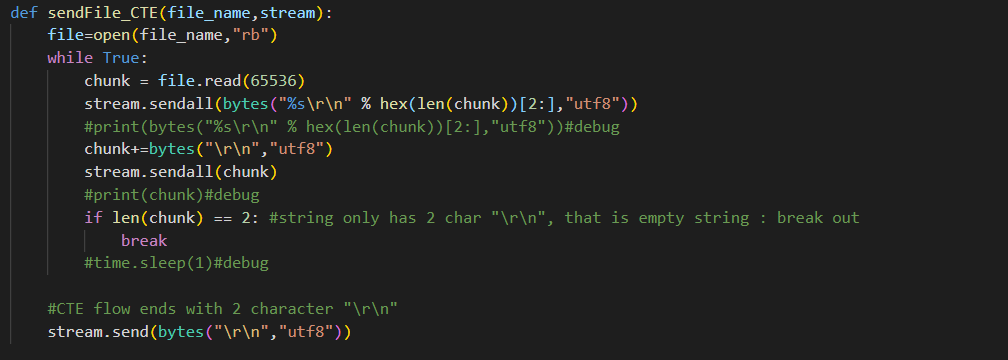
\includegraphics[scale=.8]{CTE implement.PNG}
    \end{center}
    \caption{Cài đặt hàm chuyển data từ file theo phương thức CTE bằng ngôn ngữ python}
    \end{figure}
\end{center}
\subsection{Method của request là POST}
Trong đồ án này, giao thức POST được sử dung trong việc nhập username và password. Khi đó, ta sẽ kiểm tra username và password, nếu đúng thì trả về response với mã 301 để bên client gửi lại request file biểu diễn thông tin theo yêu cầu đề bài, lúc này lại trở về việc giải quyết method GET như trên. Trượng hợp nhập username và password sai, ta sẽ gửi thông điệp 404 sẽ được trình bày ở phần tiếp theo. 
\begin{center}
    \begin{figure}[H]
    \begin{center}
     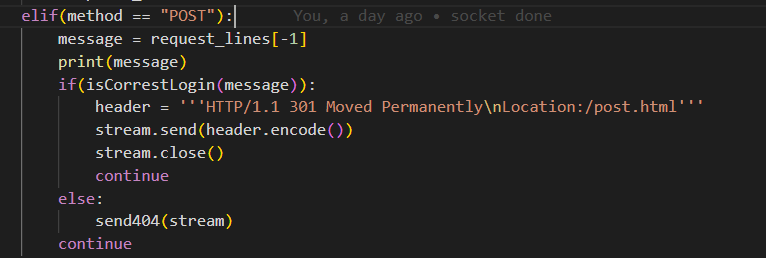
\includegraphics[scale=.8]{POST implement.PNG}
    \end{center}
    \caption{Cài đặt xử lý method POST}
    \end{figure}
\end{center}
\subsection{404 - Notfound Response}
Ngoài việc thay đổi dòng header và mặc định gửi dữ liệu file html trình chiếu trang 404, 404 response không có sự thay đổi quá nhiều so với response GET.

\begin{center}
    \begin{figure}[H]
    \begin{center}
     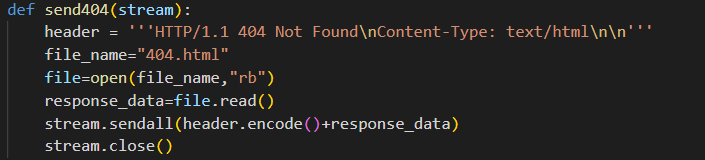
\includegraphics[scale=.8]{404 implement.PNG}
    \end{center}
    \caption{Cài đặt gửi 404 response}
    \end{figure}
\end{center}

\chapter{Phân việc}
\begin{longtable}[c]{|l|l|l|}
\hline
Công việc      & Nguyễn Hoàng Anh Kiệt     & Vũ Công Duy               \\ \hline
\endhead
%
Code socket    &                           & \cellcolor[HTML]{FCFF2F}x \\ \hline
Code front-end & \cellcolor[HTML]{FCFF2F}x &                           \\ \hline
Viết báo cáo   &                           & \cellcolor[HTML]{FCFF2F}x \\ \hline
Làm video demo & \cellcolor[HTML]{FCFF2F}x &                           \\ \hline
\caption{Bảng phân công}
\label{tab:my-table}\\
\end{longtable}
\begin{thebibliography}{3}
\bibitem{1} James F. Kurose. {\it Computer Networking: A Top-Down Approach}. 2016.
\bibitem{2} David .{\it Python Network Programming}. Thu Jun 17 19:49:58 2010.
\bibitem{3}{\it https://developer.mozilla.org/en-US/docs/Web/HTTP/Headers/Transfer-Encoding}.

\end{thebibliography}
\end{document}